%!TEX encoding = UTF-8 Unicode
%!TEX TS-program = pdflatex

%%% --- PREAMBLE --- %%%

\documentclass[a4paper,11pt]{article}

\usepackage[italian]{babel}
\usepackage[left=2cm,right=2cm,top=2cm,bottom=2cm]{geometry}
\usepackage[T1]{fontenc} % OT1: basic, T1: western, T3 and T5: exotic, T4: lots of characters but WORSE READABILITY
\usepackage[utf8x]{inputenc} % utf8x supports more characters than utf8
\usepackage{graphicx} % import PNG, JPG and PDF with \includegraphics
\usepackage[usenames,table]{xcolor} % \color
\usepackage{amssymb}
\usepackage{amsmath}
\usepackage{amsfonts}
\usepackage{mathtools} % (!! PLACE BEFORE hyperref !!)
\usepackage{xfrac} % \sfrac
\usepackage{cancel} % \cancel \cancelto
\usepackage{hyperref} % interactive links in TOC, URLs and references
% Bob \usepackage[version=3]{mhchem} % \ce (chemical formula)
\usepackage{siunitx} % \num \si \SI
\usepackage{alltt} % {alltt} (like verbatim but with commands)
\usepackage{moreverb} % {listing}
\usepackage{listings} % {lstlisting}
\usepackage[overload]{textcase} % fixes \MakeUppercase and \MakeLowercase
\usepackage[normalem]{ulem} % \uline \uwave \sout \xout
\usepackage{enumerate} % adds options for {enumerate}
\usepackage{paralist} % inline lists with {inparaenum}
\usepackage[official]{eurosym} % \euro
\usepackage{tabu} % {tabu} (like {tabular} with improvements)
\usepackage{layout} % layout description
\usepackage{multicol} % {multicols}
\usepackage{lipsum} % filling text generator with \lipsum
\usepackage[section]{placeins} % inhibits float figures from trepassing a section boundary
\usepackage{subfig} % \subfloat to be used inside {figure}
\usepackage{wrapfig} % {wrapfigure} (like {figure} but allows text to flow on its sides)
\usepackage{ifthen} % \ifthenelse
\usepackage{calc}
\usepackage{array}
\usepackage{multirow}
\usepackage{booktabs} % \toprule, \midrule, \bottomrule

\graphicspath{ {../Figs-Tabs/} } % graphics search directories
\setcounter{tocdepth}{1} % -1: part, 0: chapter, 1: section, 2: subsection, 3: subsubsection

\lstset{ %
	language=C,
	deletekeywords={},
	morekeywords={},
	backgroundcolor=\color{white},
	basicstyle=\ttfamily\small,
	commentstyle=\color{teal},
	keywordstyle=\color{magenta},
	stringstyle=\color{purple},
	identifierstyle=\color{violet!80!black},
	numbers=left,
	numbersep=7pt,
	numberstyle=\scriptsize\sffamily\color{gray},
	stepnumber=1,
	breakatwhitespace=false,
	breaklines=true,
	keepspaces=true,
	showspaces=false,
	showstringspaces=false,
	showtabs=false,
	tabsize=2,
	captionpos=none,
}

\newcommand{\swaphmargins}{
\newlength{\tmplength}
\setlength{\tmplength}{\oddsidemargin}
\setlength{\oddsidemargin}{\evensidemargin}
\setlength{\evensidemargin}{\tmplength}}

\newcommand{\setdispacing}[1][0pt]{\setlength{\abovedisplayskip}{#1}
\setlength{\belowdisplayskip}{#1}
\setlength{\abovedisplayshortskip}{#1}
\setlength{\belowdisplayshortskip}{#1}}

\newcommand{\inv}[1]{\frac{1}{#1}}
\newcommand{\dd}{\mathrm{d}}
\newcommand{\deriv}[2][x]{\frac{\dd #2}{\dd #1}}
\newcommand{\derivn}[3][x]{\frac{\dd^{#2}#3}{\dd{#1}^{#2}}}
\newcommand{\pardv}[2][x]{\frac{\partial #2}{\partial #1}}
\newcommand{\pardvn}[3][x]{\frac{\partial^{#2}#3}{\partial{#1}^{#2}}}
\newcommand{\integ}[2][x]{\int #2\,\dd #1}
\newcommand{\invinteg}[2][x]{\int\frac{\dd #1}{#2}}
\newcommand{\dinteg}[4]{\int_{#1}^{#2}#3\,\dd #4}
%\renewcommand{\arcsin}{\operatorname{asin}}
%\renewcommand{\arccos}{\operatorname{acos}}
%\renewcommand{\arctan}{\operatorname{atan}}
\DeclareMathOperator{\arccot}{arccot}
\newcommand{\vel}{\vee}
\newcommand{\et}{\wedge}

\newcommand{\fwhm}{\text{FWHM}}
\newcommand{\hwhm}{\text{HWHM}}

\newcommand{\ndr}[1]{\footnote{#1 (n.d.r.)}}
\newcommand{\fig}[1]{figura (\ref{fig:#1})} %inserting reference to figures
\newcommand{\tab}[1]{tabella (\ref{tab:#1})} % inserting reference to tables
\newcommand{\eqn}[1]{equazione \eqref{eq:#1}} % inserting reference to equation
\newcommand{\dof}{\text{ dof}} % degrees of freedom
\newcommand{\paral}{\mathbin{\|}} % impedance parallel
\DeclareSIUnit\deca{decade} % decade unit definition for use in siunitx

\newcommand{\insertpart}[2]{\input{#1}}

\newcommand{\p}{\footnote{\textbf{valore placeholder}}}
\sisetup{%
	separate-uncertainty = true,
	per-mode = symbol,
	bracket-numbers = false,
	multi-part-units = single,
	table-number-alignment = center,
	range-phrase = \text{--},
	range-units = brackets,
	output-complex-root =  \text{\ensuremath{j}},
	table-figures-decimal = 3,
	table-figures-exponent = 0,
	table-figures-integer = 2,
	table-figures-uncertainty = 2,
}

%%% --- DOCUMENT --- %%%


%%%%% SIunitX example use:
% \si{\kilo\volt\per\meter\squared} -> kV/m^2
% \SI{1.222 (34)}{\joule\second}    -> 1.222 +- 0.034 Js
% \SI{1.222 \pm 0.034}{\nF}         -> 1.222 +- 0.034 nF
% use it plz

\author{Gruppo BF \\ Roberto Ribatti, Thomas Giannoni, Valerio Lomanto}
\title{Esercitazione N.12: Flip-Flop e contatori.}
\date{4 aprile 2017}

\begin{document}
\maketitle
\begin{abstract}
		In questa esperienza sono stati realizzati ed analizzati dei circuiti logici sequenziali.
		Nella fattispecie: \begin{itemize} 
			\item un FLIP-FLOP D-LATCH
			\item dei divisori di frequenza binari 
			\item uno shift register con D-Latch
			\item un generatore di sequenze pseudo-casuali
		\end{itemize}
\end{abstract}
\section{Strumentazione}
	In tale esperienza sono state impiegate le seguenti componenti:\begin{itemize}
		\item Alcuni circuiti integrati \begin{enumerate}
			\item 2 IC SN74LS74 (Quad NAND Gate)
			\item 1 IC SN74LS93 (4-bit binary counter)
			\item 2 IC SN74LS74 (Dual D-Latch)
			\item 1 IC SN74LS86 (Quad XOR Gate)
		\end{enumerate}
		\item 1 DIP Switch a 4 interruttori
		\item 1 pulsante a doppio contatto
		\item 4 diodi LED
		\item il circuito ipulsatore basato su Arduino realizzato nell'esperienza N.10
		\item un multimetro digitale impiegato per misurare le componenti circuitali e le tensioni in continua
		\item un oscilloscopio digitale; impiegato per osservare le forme d'onda dei segnali ottenuto;per misurare i ritardi temporali e le quantità dinamiche
		\item un generatore di funzioni, quale sorgente dei nostri segnali in ingresso
	\end{itemize}
\section{Flip-Flop D-Lantch}
	per realizzare un flip-flop D-Latch (\figurename{ \ref{f:D-Latch1}}) non disponendo di porte NOT, è stato montato il circuito in \figurename{ \ref{f:D-Latch2}} impiegando le 
	porte NAND in dotazione.
	\begin{figure}[hb]
		\centering
		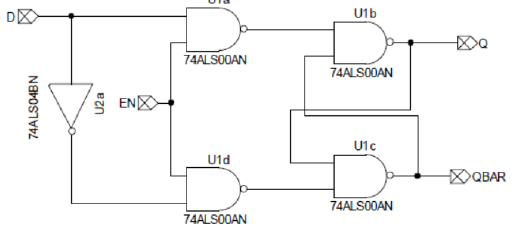
\includegraphics[scale=0.75]{../Figs-Tabs/D-Latch1.png}
		\caption{Rappresentazione di un circuito Flip-Flop D-Lantch}
			\label{f:D-Latch1}
	\end{figure}
	
	\begin{figure}[htb]
		\centering
		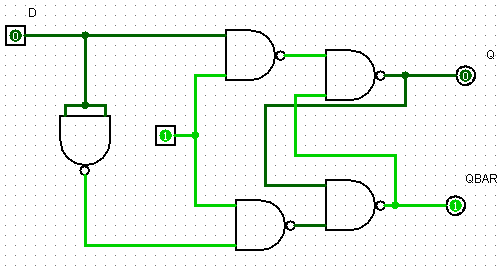
\includegraphics[scale=0.75]{../Figs-Tabs/D-Latch2.png}
		\caption{Rappresentazione del circuito Flip-Flop D-Lantch montato.
		Non disponedo di un IC SN74LS04 o analoghi la porta NOT è stata realizzata impiegando una porta NAND.}
	\label{f:D-Latch2}
	\end{figure}
	L'ingresso D del circuito è stato collegato all'ingresso Y1 dell'impulsatore basato su arduino,
	mentre l'ingresso di ENABLE è stato collegato al pulsante a doppio contatto.
	Si è inoltre fornita una tensione di alimentazione continua $V_{cc}=$\SI{4645965454 \pm 0.01}{\volt}\p.
	
	Per la verifica del funzionamento circuitale si è andati a verificare la tabella di verità riportata in \tablename{ \ref{t:D-Lantch}}.
	\begin{table}[htb]
		\centering
		\begin{tabular}{ssss}
			\toprule
			\text{ingresso $D$} & \text{ingresso $En$ }&\text{ uscita $Q$ }&\text{ uscita $\overline{Q}$}\\
			\midrule
			0 & 0 & Q_{precedente} & {\overline{Q}}_{precedente}\\
			1 & 0 & Q_{precedente} & {\overline{Q}}_{precedente}\\
			0 & 1 & 0 & 1\\
			1 & 1 & 0 & 0\\
			\bottomrule
		\end{tabular}
	\caption{tabella di verità di un Flip-Flop D-Lantch.
	Con il pedice 'precedente' si intende che lo stato non cambi e permanga nello stato in cui si trovava indipendentemente dall'ingresso $D$.}
	\label{t:D-Lantch}
	\end{table}
	La verifica si è composta in due fasi.
	Una prima fase qualitativa in cui si è verificata la tabella di verità attraverso i diodi LED; per fare ciò sono state montate delle resistenze per limitare la richiesta di corrente 
	$R_{1}=$\SI{330 \pm 1110}{\ohm}\p e $R_{2}=$\SI{330 \pm1110}{\ohm}\p rispettivamente precedentemente all'uscita $Q$ e all'uscita $\overline{Q}$.
	
	Ed uscita una seconda fase in cui si sono acquisite le tensioni osservabili 
	sulle uscite $Q$ e $\overline{Q}$ in funzione degli ingressi $D$ ed $En$. 
	$$nota-per-noi-ha-senzo-fare-come-nella-scorsa?-o-a-interruttore?$$
	
	Per fare ciò si è sostituito al ingresso si $En$ l'interruttore all'ingresso 
	$Y2$ dell'impulsatore. Essendo 	$Y1$ e 	$Y2$ sfasati di circa \ang{90}, in un periodo tali ingressi assumerebbero tutte le possibili permutazioni di un ingresso a 2 bit.
	
	Si riportano le acquisizioni ottenute in \figurename{ \ref{o:D-Latch}}	
	\begin{figure}[htb]
			\centering
			\subfloat[acquisizione delle tensioni in ingresso nel ciruito D-Leach; $D$ (ch1) ed $En$ (ch2)]{
			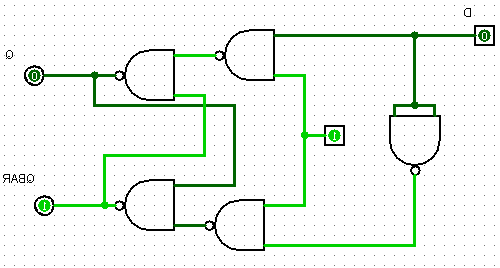
\includegraphics[scale=0.35]{../Figs-Tabs/placeholder.png}
			\label{f:ing}
		}
		\subfloat[acquisizione uscita $Q$ (ch2) e della tensione in ingresso $D$ (ch1)]{
			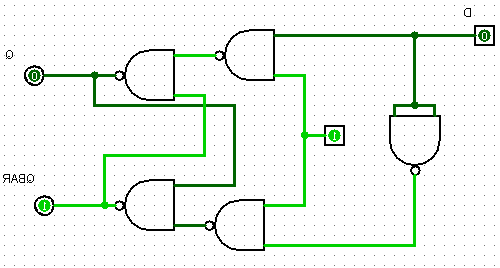
\includegraphics[scale=0.35]{../Figs-Tabs/placeholder.png}
			\label{f:sci}
		}\\
		\subfloat[acquisizione uscita $\overline{Q}$ (ch2) e della tensione in ingresso $D$ (ch1)]{
		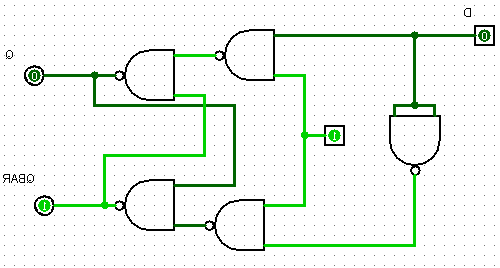
\includegraphics[scale=0.35]{../Figs-Tabs/placeholder.png}
		\label{f:sci2}
	}
	\subfloat[acquisizione uscita $Q$ (ch2) e della tensione in uscita da $\overline{Q}$  (ch1)]{
	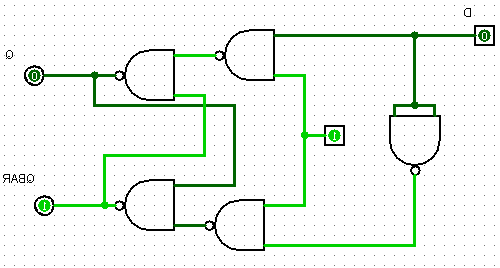
\includegraphics[scale=0.35]{../Figs-Tabs/placeholder.png}
	\label{f:sci3}
}
		\caption{acquisizioni delle schermate impiegate per la verifica di \tablename{ \ref{t:D-Lantch}}.}
		\label{o:D-Latch}
	\end{figure}
\paragraph{Misura dei tempi di ritardo}
	Essendo il circuito logico montato un sistema a più livelli
	si è assunto che i tempi di ritardo tra il segnale in ingresso e quelli in uscita non risultino trascurabili.
	
	Si è pertanto proceduto ad una misura dei tempi di propagazione per il fronte di salita e discesa del segnale.
	Per fare ciò è stata fissata un onda quadra di frequenza $f=$\SI{1690\pm 500000}{\hertz}\p  e tensione picco-picco $V_{pp}=$\SI{5 \pm 400000}{\volt}\p,
	, tali valori sono stati misurati attraverso i cursori dell'oscilloscopio
	\footnote{Per l'incertezza associata a tali misure è stata presa l'incertezza dovuta al posizionamento dei cursori. Si segnala che l'incertezza di calibrazione dell'oscilloscopio non è stata conteggiata in tali misure ed è da considerarsi scorporata da tali incertezze. }.
	Tali onda è stata impiegata quale  segnale per l'ingresso $D$, mentre per la porta $En$ impiegando l'interruttore è stato posto il segnale sull'$1$ logico.
	Visualizzando l'andamento del segnale in $D$ e nelle uscite $Q$ e $\overline{Q}$
	sono stati misurati i seguenti ritardi:\\
	\begin{center}
		$ \Delta t_{Q,salita}=$\SI{20.8 \pm 0.6}{\nano \sec}\p \qquad $ \Delta t_{Q,discesa}=$\SI{60 \pm 0.6}{\nano \sec}\p\\
			$ \Delta t_{\overline{Q},salita}=$\SI{20.8 \pm 0.6}{\nano \sec}\p \qquad $ \Delta t_{\overline{Q},discesa}=$\SI{60 \pm 0.6}{\nano \sec}\p\\
	\end{center}
	
		\begin{figure}[htb]
		\centering
		\subfloat[acquisizione uscita $Q$ (ch2) e della tensione in ingresso $D$ (ch1)]{
			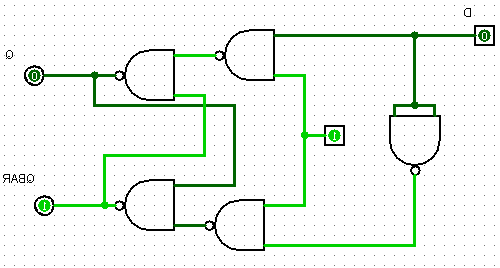
\includegraphics[scale=0.35]{../Figs-Tabs/placeholder.png}
			\label{f:t1}
		}\\
		\subfloat[acquisizione uscita $\overline{Q}$ (ch2) e della tensione in ingresso $D$ (ch1)]{
			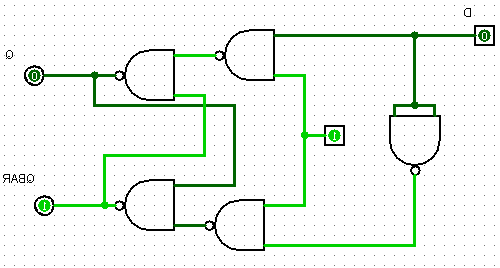
\includegraphics[scale=0.35]{../Figs-Tabs/placeholder.png}
			\label{f:t2}
		}\\
		\subfloat[acquisizione uscita $Q$ (ch2) e della tensione in uscita da $\overline{Q}$  (ch1)]{
			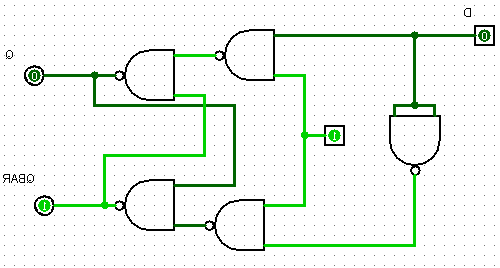
\includegraphics[scale=0.35]{../Figs-Tabs/placeholder.png}
			\label{f:sci3}
		}
		\caption{acquisizioni delle schermate impiegate per la misura dei tempi di ritardo del circuito in \figurename{ \ref{f:D-Latch2}}.}
		\label{o:t-D-Latch}
	\end{figure}
	
	Come è possibile osservare da i valori ottenuti $\Delta t_{\overline{Q},salita} \sim \Delta t_{{Q},discesa}$ e $\Delta t_{\overline{Q},discesa} \sim \Delta t_{{Q},salita}$; ciò risulta compatibile con le attese, essendo entrambe le uscite poste sul solito livello ed una l'inverso dell'altro.
	\paragraph{alcune analisi sulla costituzione ciruitali }
	Come riportato in \figurename{ \ref{f:D-Latch1}} per la realizzazione del Flip-Flop D-Latch in esame si è impiegato una porta NOT;
	tale porta svolge la la funzione di inviare agli ingressi del flip-flop D-latch valori opposti; evitando pertanto di inviare a entrambi gli ingressi contemporaneamente $1$ logico e quindi la zona "proibita".
	Se il sistema fosse in tale stato una successiva variazione del segnale in ingresso porterebbe a variazioni non prevedibili delle uscite.
	
	Si segnala inoltre che essendo le porte NAND impiegate basate su logica TTL quando esse non risultino collegate a terra si ottiene in uscita alla porta un segnale corrispondente allo stato HIGH; pertanto l'ingresso $En$ risulta essere attivo per
	segnali in ingresso, in $En$, corrispondenti allo stato LOW.
	\section{Divisori in frequenza}
	Per realizzare un circuito divisore di frequenza binario come da richieste si è andati a nontare il circuito in \figurename{ \ref{f:div1}}.
	
	Per la realizzazione circuitale sono state impiegate le seguenti  resistenze di limitazione di corrente:
	\\$R_{1}=$\SI{330 \pm 44444}{\ohm}\p \\
	$R_{2}=$\SI{330 \pm 44444}{\ohm}\p \\
	$R_{3}=$\SI{330 \pm 44444}{\ohm}\p \\
	$R_{4}=$\SI{330 \pm 44444}{\ohm}\p \\
	e l'IC SN74LS93; ovvero un ripple counter composto di quattro flip-flop JK.
	L'ingresso $R0$ è stato collegato a terra in modo da garantire un ingresso alla porta NAND posto sull'$1$ logico.
	Essendo i Flip-Flop dell'IC SN74LS93 posti in configurazione $Master-slave$ 
	si attende che per ognuno di essi si ottenga una divisione per 2 del segnale di clock in ingresso; ottenendo pertanto frequenze rispettivamente 1/2, 1/4, 1/8 ed 1/16 della frequenza di
	clock iniziale.
	\begin{figure}[htb]
		\centering
		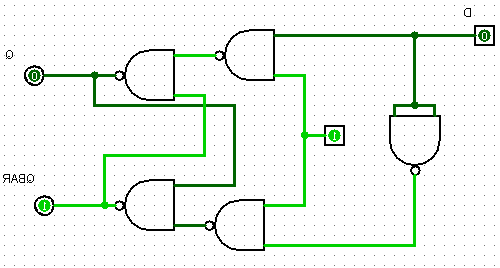
\includegraphics[scale=0.5]{../Figs-Tabs/placeholder.png}
		\caption{schema circuitale del divisore di frequenza binario realizzato.}
		\label{f:div1}
	\end{figure}
\paragraph{verifica funzionamento contatore.}
	Per tale verifica attraverso il generatore di onde quadre in dotazione 
	si è inviata una frequenza di clock al primo Flip-Flop $f_{clock,1}=$\SI{3567 \pm 0.1}{\hertz}\p$\sim$\SI{1}{\hertz};
	attraverso l'accensione e lo spegnimento dei diodi LED montati è stato verifico che il circuito riproducesse la codifica binaria da 0 a 15 nella corretta sequenza.
\paragraph{verifica funzionamento divisore e misura dei tempi di ritardo.}
	Effettuata la verifica precedente si è posta $f_{clock,1}=$\SI{76 \pm 2}{ \kilo \hertz}\p
\end{document}
	
	